% !TEX program = pdflatex
% Standalone system-model figure for DynaQGNN-IDS paper.
% Compile: pdflatex fig-system-model.tex  ->  fig-system-model.pdf
% Tuan thu Gem 2 (The TikZ Architect) conventions.

\documentclass[tikz,border=10pt]{standalone}

\usepackage[utf8]{inputenc}
\usepackage[T1]{fontenc}
\usepackage{tikz}
\usepackage{pgfplots}
\pgfplotsset{compat=1.18}

\usetikzlibrary{arrows.meta, positioning, calc, shapes, shapes.geometric,
                fit, backgrounds, shadows.blur, decorations.pathreplacing,
                decorations.markings}

% ===== Palette =====
\definecolor{primary}{RGB}{11, 95, 165}     % accent blue
\definecolor{secondary}{RGB}{184, 134, 11}  % accent gold
\definecolor{success}{RGB}{46, 139, 87}     % green
\definecolor{danger}{RGB}{178, 34, 34}      % red
\definecolor{neutral}{RGB}{96, 106, 115}    % gray
\definecolor{skyfill}{RGB}{232, 241, 250}
\definecolor{groundfill}{RGB}{240, 240, 235}

% ===== Styles =====
\tikzset{
  sat/.style={
    draw=primary, thick, fill=primary!15,
    rounded corners=3pt, minimum width=1.1cm, minimum height=0.55cm,
    font=\sffamily\tiny, align=center,
    drop shadow={blur shadow={shadow xshift=0.5pt, shadow yshift=-0.5pt}}
  },
  sat_det/.style={
    draw=success, very thick, fill=success!25,
    rounded corners=3pt, minimum width=1.1cm, minimum height=0.55cm,
    font=\sffamily\tiny\bfseries, align=center,
    drop shadow={blur shadow={shadow xshift=0.5pt, shadow yshift=-0.5pt}}
  },
  ue/.style={
    draw=neutral, thick, fill=white,
    rounded corners=2pt, minimum width=0.8cm, minimum height=0.4cm,
    font=\sffamily\tiny, align=center
  },
  ueblock/.style={
    draw=neutral!60, thick, fill=neutral!8,
    rounded corners=5pt, inner sep=5pt,
    font=\sffamily\small, align=center
  },
  gateway/.style={
    draw=primary, very thick, fill=primary!25,
    shape=trapezium, trapezium left angle=70, trapezium right angle=110,
    minimum width=1.2cm, minimum height=0.7cm,
    font=\sffamily\small\bfseries, align=center,
    drop shadow={blur shadow={shadow xshift=0.5pt, shadow yshift=-0.5pt}}
  },
  attacker/.style={
    draw=danger, very thick, fill=danger!15,
    regular polygon, regular polygon sides=6,
    minimum width=0.9cm, font=\sffamily\small\bfseries,
    drop shadow={blur shadow={shadow xshift=0.5pt, shadow yshift=-0.5pt}}
  },
  isl/.style={-Stealth, thick, primary, dashed},
  uplink/.style={-Stealth, thick, neutral},
  downlink/.style={-Stealth, thick, neutral},
  attack/.style={-Stealth, ultra thick, danger, decorate,
                 decoration={snake, amplitude=0.6mm, segment length=3mm}},
  layerlabel/.style={font=\sffamily\footnotesize\itshape, neutral},
}

\begin{document}
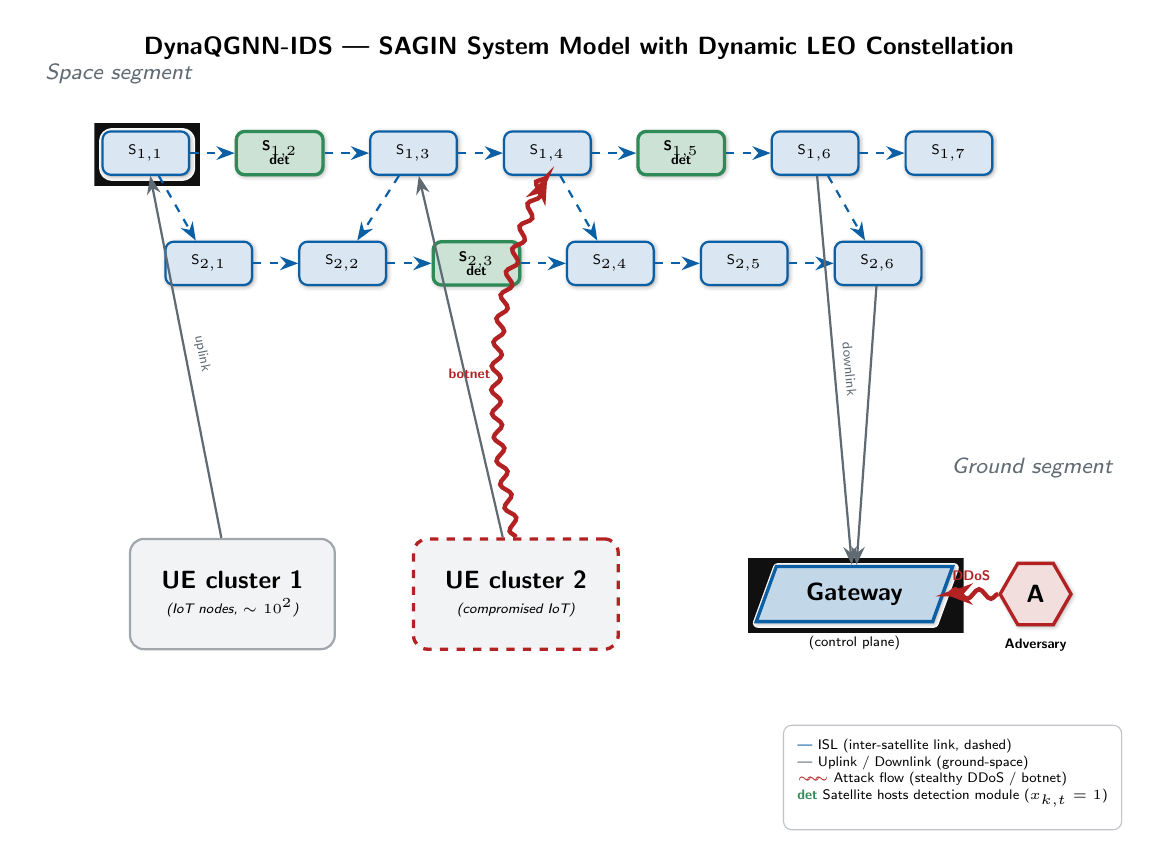
\begin{tikzpicture}[node distance=1cm]

  % ============ SKY LAYER (LEO constellation) ============
  \begin{scope}[on background layer]
    \fill[skyfill, rounded corners=4pt]
      (-1, 4.5) rectangle (13, 8.2);
  \end{scope}

  \node[layerlabel, anchor=west] at (-0.9, 8.0) {Space segment};

  % Row 1 of satellites (plane A)
  \node[sat]     (s11) at ( 0.5, 7.0) {S$_{1,1}$};
  \node[sat_det] (s12) at ( 2.2, 7.0) {S$_{1,2}$\\[-1pt]{\tiny\bfseries det}};
  \node[sat]     (s13) at ( 3.9, 7.0) {S$_{1,3}$};
  \node[sat]     (s14) at ( 5.6, 7.0) {S$_{1,4}$};
  \node[sat_det] (s15) at ( 7.3, 7.0) {S$_{1,5}$\\[-1pt]{\tiny\bfseries det}};
  \node[sat]     (s16) at ( 9.0, 7.0) {S$_{1,6}$};
  \node[sat]     (s17) at (10.7, 7.0) {S$_{1,7}$};

  % Row 2 (plane B)
  \node[sat]     (s21) at ( 1.3, 5.6) {S$_{2,1}$};
  \node[sat]     (s22) at ( 3.0, 5.6) {S$_{2,2}$};
  \node[sat_det] (s23) at ( 4.7, 5.6) {S$_{2,3}$\\[-1pt]{\tiny\bfseries det}};
  \node[sat]     (s24) at ( 6.4, 5.6) {S$_{2,4}$};
  \node[sat]     (s25) at ( 8.1, 5.6) {S$_{2,5}$};
  \node[sat]     (s26) at ( 9.8, 5.6) {S$_{2,6}$};

  % ISL horizontal (intra-plane)
  \foreach \a/\b in {s11/s12, s12/s13, s13/s14, s14/s15, s15/s16, s16/s17,
                     s21/s22, s22/s23, s23/s24, s24/s25, s25/s26} {
    \draw[isl] (\a) -- (\b);
  }
  % ISL vertical (inter-plane)
  \foreach \a/\b in {s11/s21, s13/s22, s14/s24, s16/s26} {
    \draw[isl] (\a) -- (\b);
  }

  % ============ GROUND LAYER ============
  \begin{scope}[on background layer]
    \fill[groundfill, rounded corners=4pt]
      (-1, -0.5) rectangle (13, 3.3);
  \end{scope}

  \node[layerlabel, anchor=east] at (12.9, 3.0) {Ground segment};

  % UE clusters (uc2 is drawn with a red dashed border to indicate
  % that some of its devices are compromised -> launch botnet flows upward)
  \node[ueblock, minimum width=2.6cm, minimum height=1.4cm]
    (uc1) at (1.6, 1.4) {\textbf{UE cluster 1}\\[-2pt]{\tiny\itshape (IoT nodes, $\sim 10^2$)}};
  \node[ueblock, minimum width=2.6cm, minimum height=1.4cm,
        draw=danger, dashed, very thick]
    (uc2) at (5.2, 1.4) {\textbf{UE cluster 2}\\[-2pt]{\tiny\itshape (compromised IoT)}};

  % Gateway
  \node[gateway] (gw) at (9.5, 1.4) {Gateway};
  \node[font=\sffamily\tiny, below=1pt of gw] {(control plane)};

  % Attacker
  \node[attacker] (atk) at (11.8, 1.4) {A};
  \node[font=\sffamily\tiny\bfseries, below=1pt of atk] {Adversary};

  % ============ LINKS (uplink, downlink, attack) ============
  % Uplinks
  \draw[uplink] (uc1) -- (s11) node[midway, sloped, above, font=\sffamily\tiny] {uplink};
  \draw[uplink] (uc2) -- (s13);

  % Downlinks
  \draw[downlink] (s16) -- (gw) node[midway, sloped, above, font=\sffamily\tiny] {downlink};
  \draw[downlink] (s26) -- (gw);

  % Two attack vectors so nothing crosses the gateway:
  %   (A) Remote DDoS: adversary --> gateway (short horizontal arrow)
  %   (B) Botnet via compromised UE cluster 2 --> detection satellite
  \draw[attack] (atk.west) -- (gw.east);
  \node[font=\sffamily\tiny\bfseries, danger, anchor=south] at ($(atk.west)!0.5!(gw.east) + (0, 0.05)$) {DDoS};

  \draw[attack] (uc2.north) to[bend left=18] (s14.south);
  \node[font=\sffamily\tiny\bfseries, danger, anchor=east] at (5.0, 4.2) {botnet};

  % ============ LEGEND ============
  \node[draw=neutral!40, fill=white, rounded corners=3pt, inner sep=5pt,
        anchor=south east, font=\sffamily\tiny, align=left]
        (legend) at (12.9, -1.6) {
    \textcolor{primary}{\textbf{---}} ISL (inter-satellite link, dashed) \\
    \textcolor{neutral}{\textbf{---}} Uplink / Downlink (ground-space) \\
    \textcolor{danger}{\textbf{$\sim\!\!\sim\!\!\sim$}} Attack flow (stealthy DDoS / botnet) \\
    \textcolor{success}{\textbf{det}} Satellite hosts detection module ($x_{k,t}=1$) \\
  };

  % Title
  \node[font=\sffamily\small\bfseries, anchor=north, align=center] at (6, 8.6)
    {DynaQGNN-IDS --- SAGIN System Model with Dynamic LEO Constellation};

\end{tikzpicture}
\end{document}
